% preambolo per doppia compilazione HTML/PDF
\ifx\pdfoutput\undefined      % compilazione htlatex
\documentclass{article}
\DeclareGraphicsExtensions{.png, .gif, .jpg}
\newcommand{\href}[2]{\Link[#1]{}{} #2 \EndLink}
\newcommand{\hypertarget}[2]{\Link[]{}{#1} #2 \EndLink}
\newcommand{\hyperlink}[2]{\Link[]{#1}{} #2 \EndLink}
\else                         % compilazione pdflatex
\documentclass{article}
\usepackage{graphicx}
\usepackage{listings}
\usepackage{fancyhdr}
\usepackage{wrapfig}
\usepackage{multirow}
\usepackage{lscape}
\usepackage{slashed}
\usepackage{color}
\usepackage{amssymb,amsmath}
\pdfpagewidth 8.5in
\pdfpageheight 11in
\setlength\textwidth{6.5in}
\setlength\textheight{8.1in}
\setlength\oddsidemargin{0in}
\setlength\evensidemargin{0in}
\setlength\topmargin{-0.6in}
\setlength\footskip{0.6in}
\setlength\headsep{0.6in}
\usepackage[hyperindex]{hyperref}
\newcommand{\percent}{\,^0\!/_0}
 \hypersetup{
    unicode=false,          % non-Latin characters in Acrobat’s bookmarks
    pdftoolbar=true,        % show Acrobat’s toolbar?
    pdfmenubar=true,        % show Acrobat’s menu?
    pdffitwindow=true,      % page fit to window when opened
    pdfauthor={Maurizio},   % author
    pdfsubject={Ungaro},    % subject of the document
    pdfnewwindow=true,      % links in new window
    colorlinks=true,        % false: boxed links; true: colored links
    linkcolor=black,        % color of internal links
    citecolor=blue,         % color of links to bibliography
    filecolor=magenta,      % color of file links
    urlcolor=blue           % color of external links
}
\fi

\font\refj     = pbkl scaled 800


\begin{document}

\pagestyle{fancy}
\renewcommand{\sectionmark}[1]{\markright{\slshape \thesection\ #1}{}}
\fancyhead[R]{\bf\rightmark}
\fancyhead[L]{LTCC n. photoelectrons study}
\fancyfoot[R]{ \sl M. Ungaro}
\fancyfoot[L]{ \sl JLAB}

\begin{flushright}
CLAS-NOTE 2013-01\\
{\small svn: https://clas12svn.jlab.org/repos/clas12/gemc/trunk/systems/clas12/ltcc/docs }\\
Version: 1.0
\end{flushright}

\vspace{1.6cm}

\begin{center}
{\Large \bf Study of Number of photo-electrons for LTCC/ECI mirrors,  UVG/Quartz PMT and LTCC window increase} \hfill \\
\vspace{0.6cm}
{  M. Ungaro} \hfill
\end{center}
\vspace{0.6cm}



\abstract{The  photo-electron yield has been calculated for different mirrors,
window and PMTs configurations for the Light Threshold Cherenkov Counter (LTCC).
The mirrors re-coating corresponds to a 40-50\% 
increase in number of photo-electrons, and the quartz PMTs provide a factor of $\sim 40\%$.
An additional $\sim 50\%$ can be achieved in the center of the LTCC by increasing the gas volume.}



\section{Introduction}

A LTCC elliptical mirror spare was sent to Evaporated Coating Inc. (ECI) to be stripped and re-coated. ECI tried to strip the existing AlMgF2 
(with poor success) and then re-coat it with AlMgF2. The resulting spare reflectivity was below 30\%. 
ECI also coated the witness sample and sample mirror resulted from AlMgF2 coating of a lexan layer.
We measured the reflectivities of the two ECI samples and an actual LTCC hyperbolic mirror used in CLAS6 experiments.
The results \cite{bib:andrew} are shown in Fig.~\ref{fig:refl}, extrapolated from $\lambda=400nm$  to $\lambda=650nm$.

When it was built originally the LTCC mirror had reflectivity very similar to the ECI sample. 
After 18 years of operation, there is a 10-15\% (absolute) degradation. Here we'll report on 
the effect of this degradation on the number of photo-electrons.

The comparison of quantum efficiency of standard glass PMT, UV glass PMT (current LTCC) and Quartz PMT
as reported by the manufacturer \cite{bib:alex}
is shown in Fig.~\ref{fig:qe}.  In this document we'll show the effect of using UV glass vs quartz PMTs 
on the number of photoelectrons detected.

Finally, part of the LTCC modifications include a bigger volume for the LTCC, accomplished with a nose extension.
We report on the number of photo-electrons gained from this modification.

\newpage


\begin{figure}[t]
	\centering
	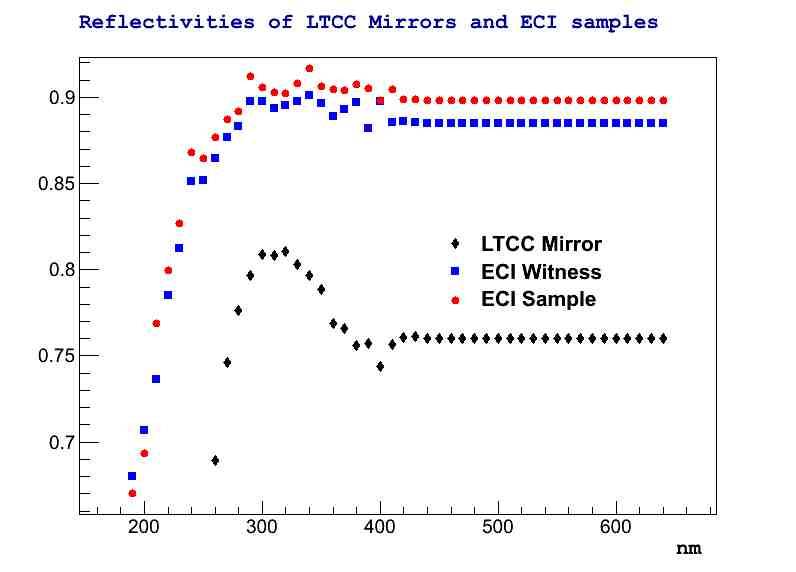
\includegraphics[width=0.7\textwidth]{img/reflectivity.jpg}
	\caption{\scriptsize Reflectivity comparison between an hyperbolic LTCC mirror used in CLAS6 and ECI samples.}
	\label{fig:refl}
\end{figure}
\begin{figure}[b]
	\centering
	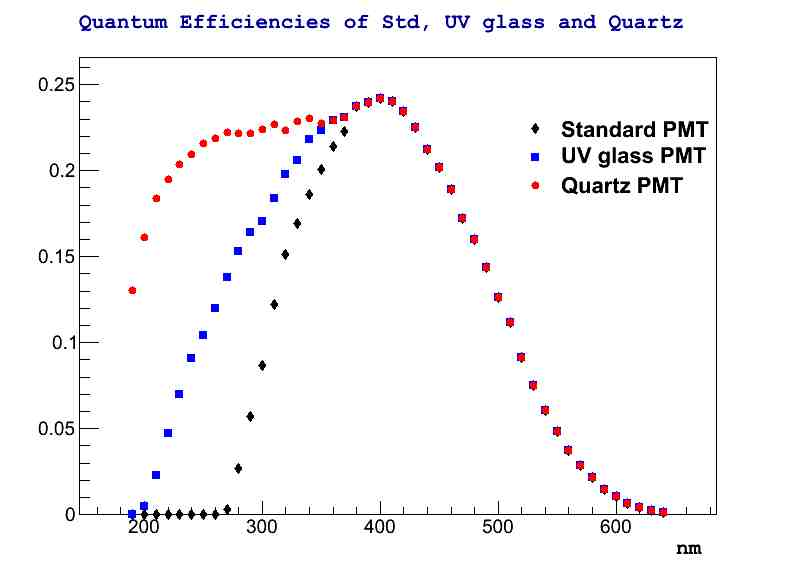
\includegraphics[width=0.7\textwidth]{img/quantum_efficiency.jpg}
	\caption{\scriptsize Quantum efficiency of standard PMT, UV glass PMT, Quartz PMT.}
	\label{fig:qe}
\end{figure}



\clearpage\newpage
\section{Number of photo-electron spectrum}

The C4F10 refraction index is shown in Fig.~\ref{fig:ri} \cite{bib:c4f10refr}. The C4F10 is transparent at all light frequency except below 220nm,
where the transparency drop to 0.99 (210$nm$), 0.805 (200$nm$), 0.262 (190$nm$).
The number of photons produced per unit path length dx of a single charged particle per unit of wavelength interval $d\lambda$ and as a function of the 
particle momentum is given by Tamm's formula \cite{bib:tamm}: 
$$
\frac{d^2N}{d\lambda dx} = \frac{2\pi\alpha}{\lambda^2}(1 - \frac{1}{\beta^2n^2(\lambda)})
$$
The number of photo-electrons spectrum per unit of length for electrons, pions and kaons using a 100\% transparent gas, 100\% efficient PMT and 
100\% reflectivity mirror is shown in Fig.~\ref{fig:spectra} (left column).
When the LTCC current mirror reflectivity, C4F10 transparency and UV glass quantum
efficiency is taken into account, the photo-electrons yiled /cm spectrum is shown in
 Fig.~\ref{fig:spectra} (middle column). If the mirrors are re-coated by ECI, the yield is seen in  Fig.~\ref{fig:spectra} (right column).
\begin{figure}[ht]
	\centering
	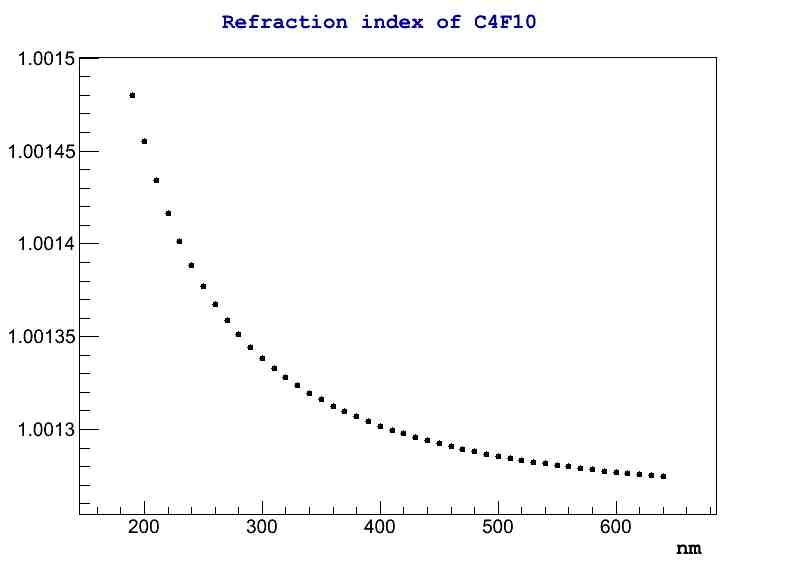
\includegraphics[width=0.9\textwidth]{img/refraction_index.jpg}
	\caption{\scriptsize C4F10 Refraction Index. Data from \cite{bib:c4f10refr}.}
	\label{fig:ri}
\end{figure}

The total number of photo-electrons as a function of particle momenta, that is given by the integral over 
the wavelength of Tamm's formula, is shown in Fig.~\ref{fig:yields} (left) for the current LTCC hardware and 
 Fig.~\ref{fig:yields} (right) using ECI re-coated mirrors and quartz PMTs. Notice the factor of 2 improvement.
 Currently the photo-electron yields by electron is about 0.3 p.e. / cm. This correspond to about 10 p.e. detected in CLAS6.
 Without hardware changes, 4 GeV pions will yield about half that amount.
 
Using the current LTCC mirror/PMT photo-electrons yields for electrons as reference, the ratio of yields for pions
using LTCC or ECI mirror and UV glass or quartz PMT is calculated and shown in Fig.~\ref{fig:ratios}.

The re-coating of the existing LTCC mirrors yield 50\% more photo-electrons. Using the quartz PMTs yields 40-50\% more
photo-electrons. The quartz PMT advantage is also  seen in Fig.~\ref{fig:quartz}.  
\vspace{1cm}
\begin{figure}[h]
	\centering
	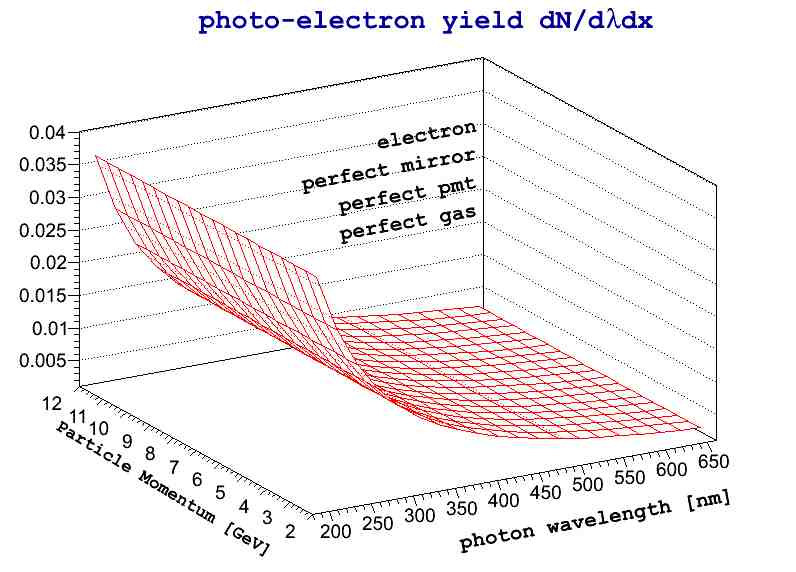
\includegraphics[width=0.3\textwidth]{img/photon_yield_spectrum_electron_gasperfect_mirrorperfect_pmtperfect.jpg}
	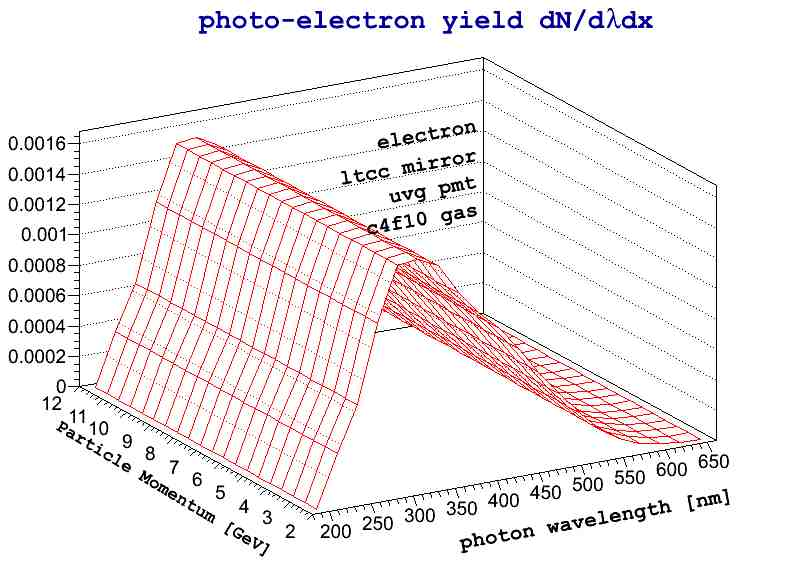
\includegraphics[width=0.3\textwidth]{img/photon_yield_spectrum_electron_gasc4f10_mirrorltcc_pmtuvg.jpg}
	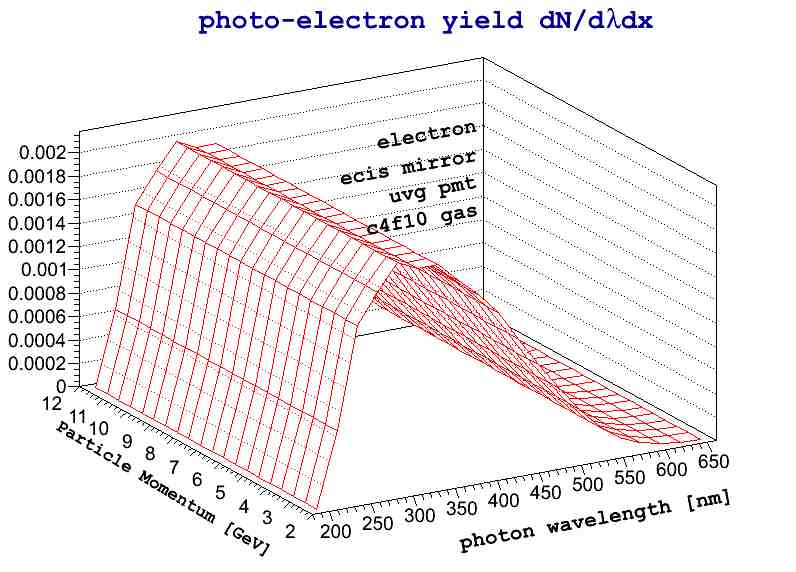
\includegraphics[width=0.3\textwidth]{img/photon_yield_spectrum_electron_gasc4f10_mirrorecis_pmtuvg.jpg}
	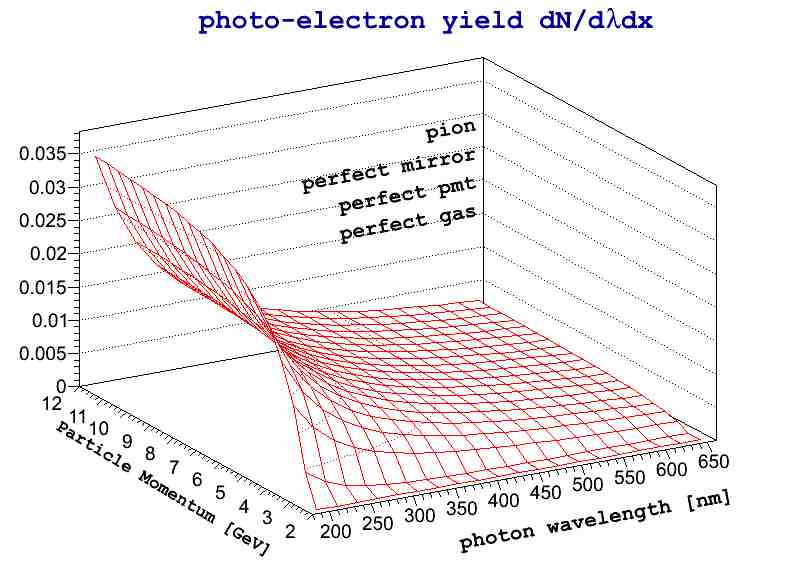
\includegraphics[width=0.3\textwidth]{img/photon_yield_spectrum_pion_gasperfect_mirrorperfect_pmtperfect.jpg}
	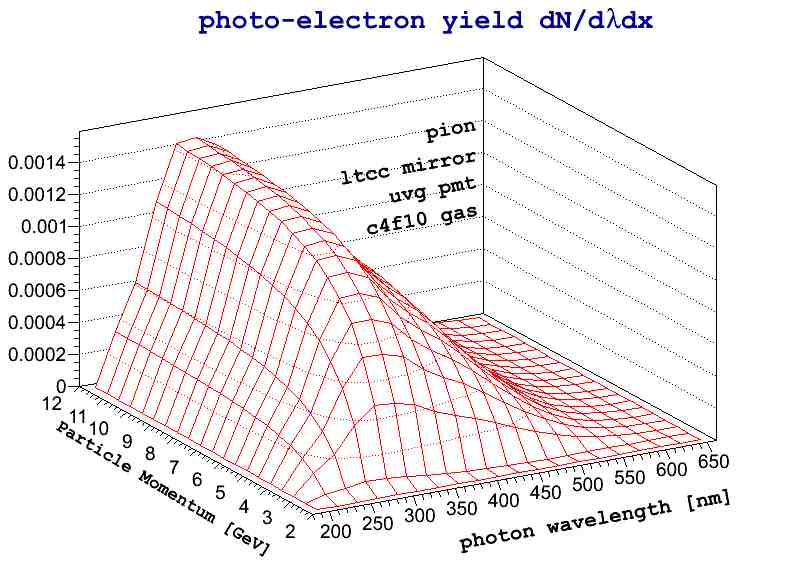
\includegraphics[width=0.3\textwidth]{img/photon_yield_spectrum_pion_gasc4f10_mirrorltcc_pmtuvg.jpg}
	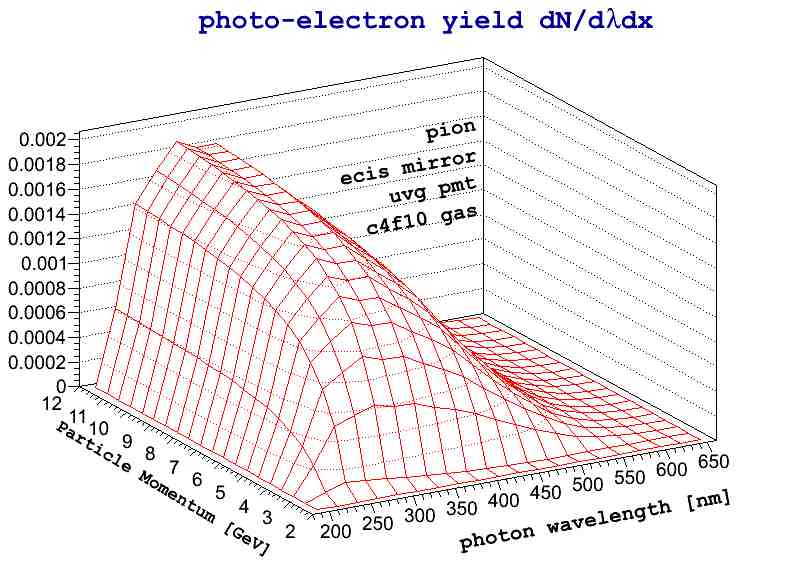
\includegraphics[width=0.3\textwidth]{img/photon_yield_spectrum_pion_gasc4f10_mirrorecis_pmtuvg.jpg}
	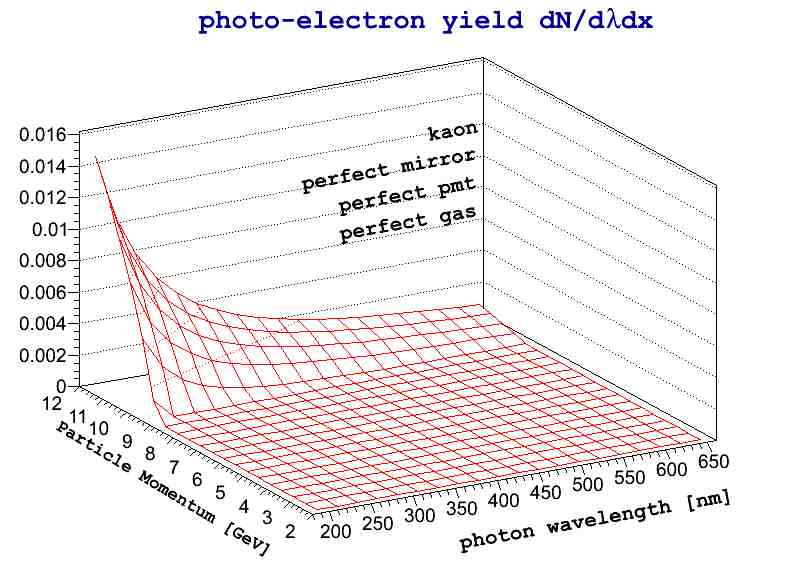
\includegraphics[width=0.3\textwidth]{img/photon_yield_spectrum_kaon_gasperfect_mirrorperfect_pmtperfect.jpg}
	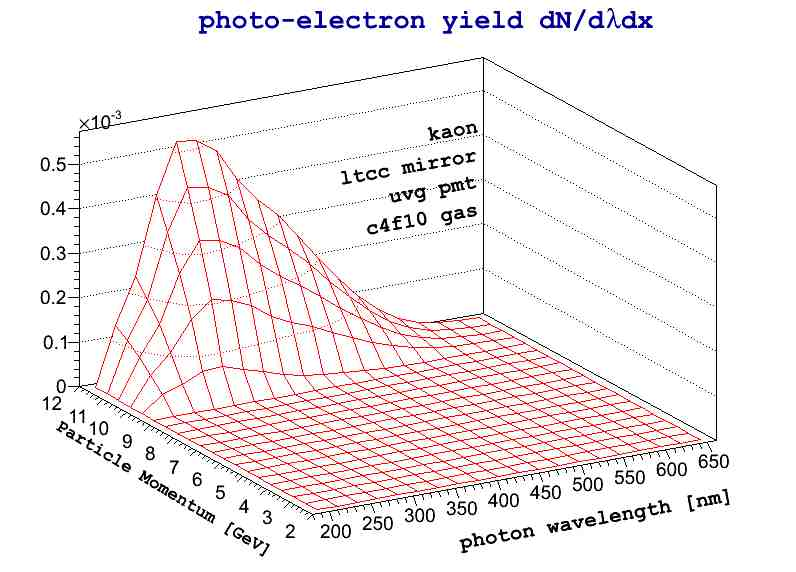
\includegraphics[width=0.3\textwidth]{img/photon_yield_spectrum_kaon_gasc4f10_mirrorltcc_pmtuvg.jpg}
	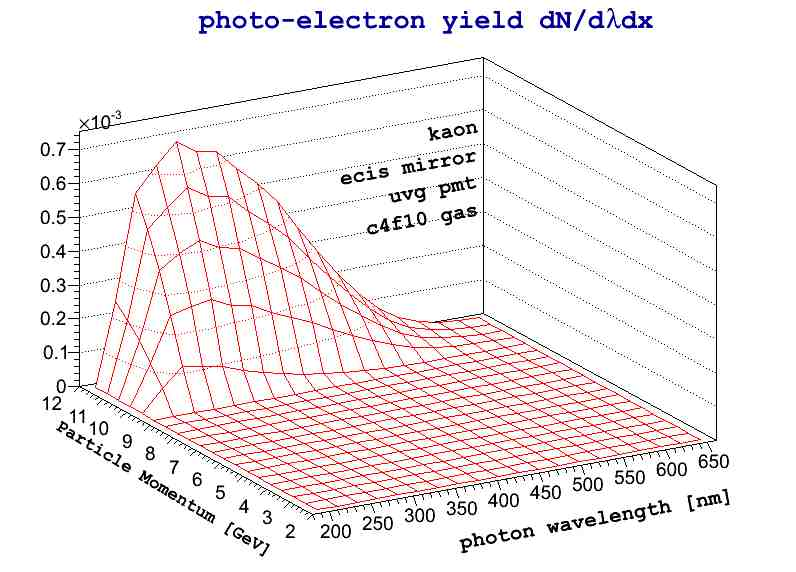
\includegraphics[width=0.3\textwidth]{img/photon_yield_spectrum_kaon_gasc4f10_mirrorecis_pmtuvg.jpg}
	\caption{\scriptsize Photo-electron Yield $\frac{d^2N}{dxd\lambda}$  as a function of wavelength and particle momenta 
	for electrons, pions and kaons. Left: if 100\% is used for reflectivity, quantum efficiency and transparency. Middle: using the current LTCC 
	mirrors and PMTs. Right: using re-coated mirrors and current LTCC PMTs.}
	\label{fig:spectra}
\end{figure}

\clearpage\newpage
\begin{figure}[ht]
	\centering
	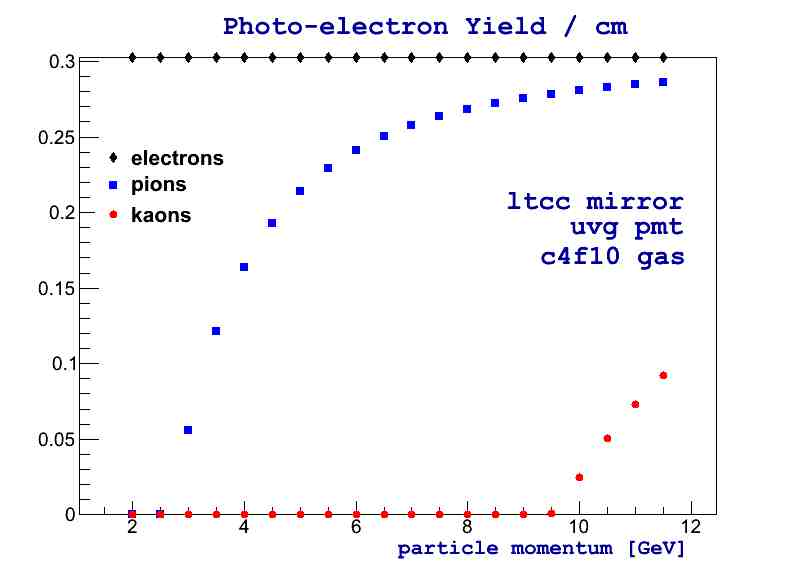
\includegraphics[width=0.48\textwidth]{img/photon_yield_gasc4f10_mirrorltcc_pmtuvg.jpg}
	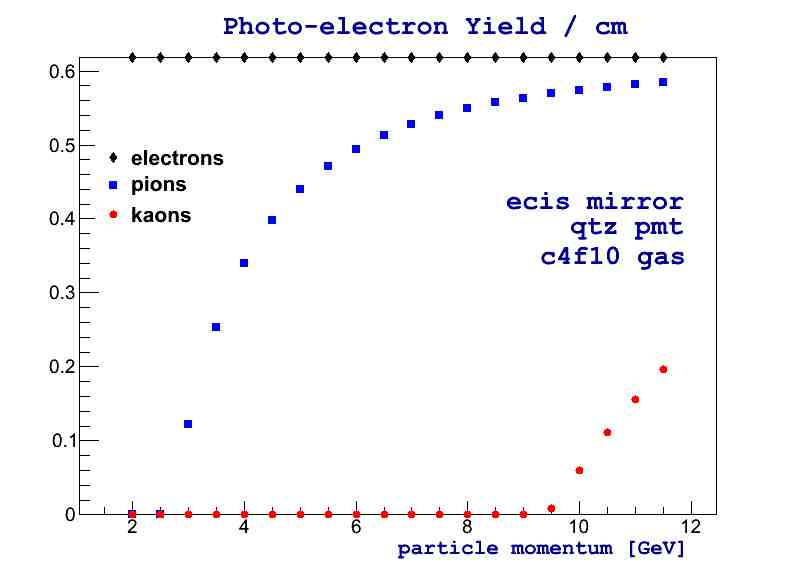
\includegraphics[width=0.48\textwidth]{img/photon_yield_gasc4f10_mirrorecis_pmtqtz.jpg}
	\caption{\scriptsize Photo-electron Yield / cm for different configurations. Left: using the current LTCC hardware. Right: using 
	improved mirrors and PMTs. The combined improvement yield a factor of 2 more photo-electrons.}
	\label{fig:yields}
\end{figure}

\begin{figure}[ht]
	\centering
	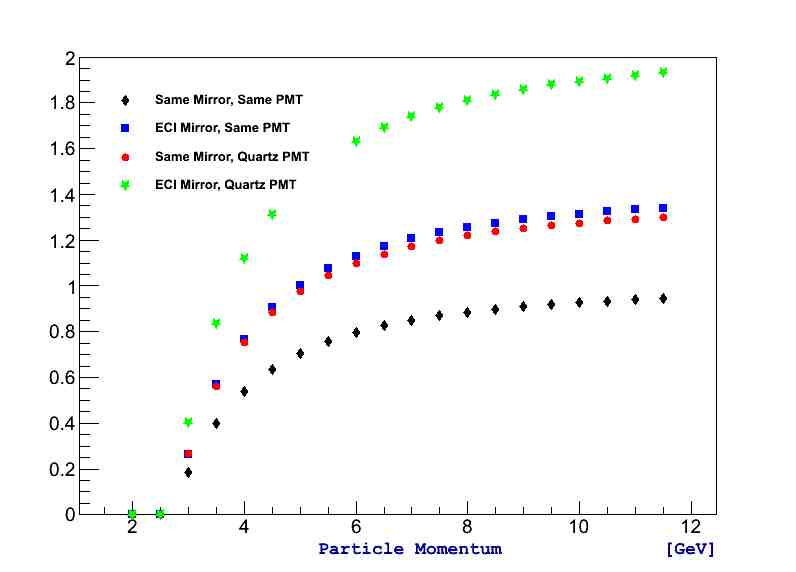
\includegraphics[width=0.58\textwidth]{img/photon_yield_ratios_pion_gasc4f10_mirrorecis_pmtqtz.jpg}
	\caption{\scriptsize Pion / Electron Photo-electrons Yield ratios for different configuration. The electron yield
	is calculated using the current hardware. Without modifications at 4GeV pions will yield half the number of photo-electrons
	that electrons currently produce. Since electrons typically yield 10 p.e., this correspond to about 5 photo-electrons.
	Both the mirror re-coating and the quartz PMT provide between 40 and 50\% improvement on the photo-electron yields.}
	\label{fig:ratios}
\end{figure}

\clearpage
\begin{figure}[ht]
	\centering
	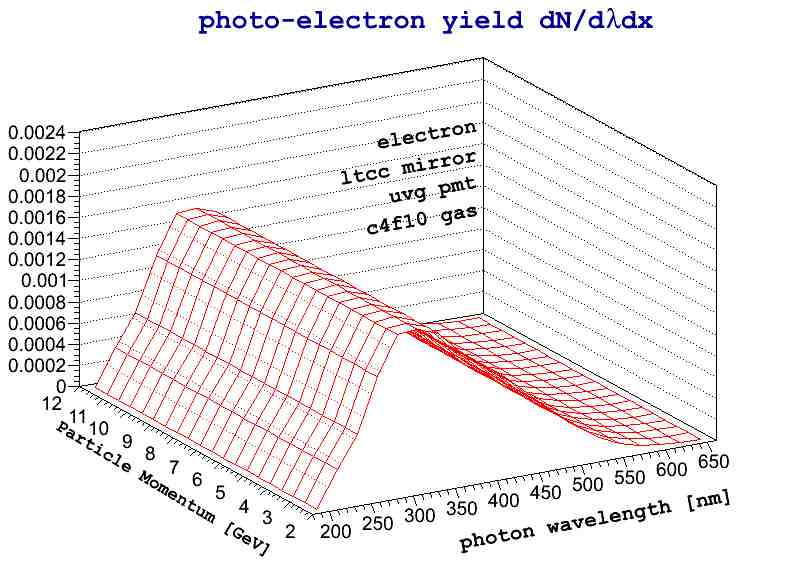
\includegraphics[width=0.8\textwidth]{img/photon_yield_spectrum_electron_gasc4f10_mirrorltcc_pmtuvg2.jpg}
	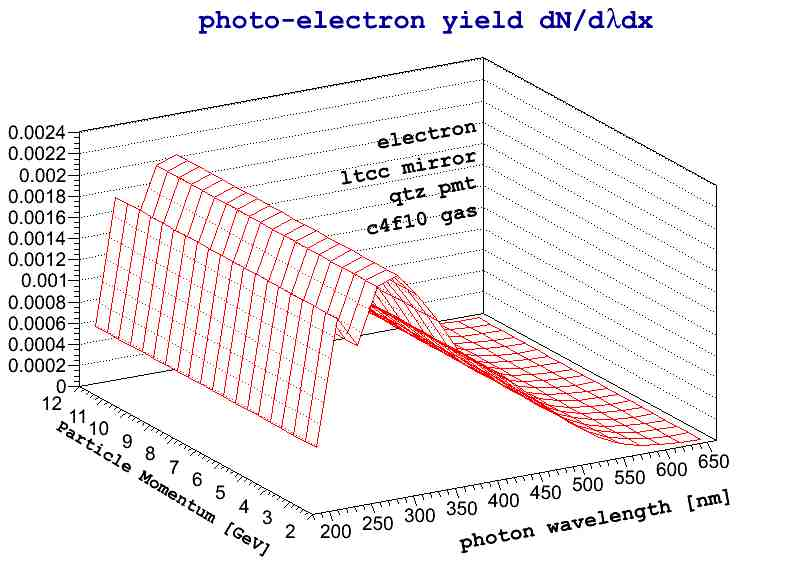
\includegraphics[width=0.8\textwidth]{img/photon_yield_spectrum_electron_gasc4f10_mirrorltcc_pmtqtz2.jpg}
	\caption{\scriptsize Photo-electron Yield $\frac{dN}{dxd\lambda}$  as a function of wavelength and particle momenta 
	for  pions. Top: using UV glass PMT. Bottom: using quartz PMTs}
	\label{fig:quartz}
\end{figure}




\clearpage\newpage
\section{Window modifications}
The LTCC box has to be modified in order to fit into the CLAS12 forward carriage, between the DCs and FTOF.
The modifications are shown in Fig.~\ref{fig:mods}: a cut of the side walls and nose to increase gas volume.
The gas volume can be increased by allowing the window on the side-wall to be loose, and inflated with C4F10. 
A nose addition can be added to further increase the volume. The increase in C4F10 gas at the center of the LTCC
is shown in Fig:~\ref{fig:window} for several configurations. With the LTCC cut very likely to happen, one can see the 
proposed 8'' nose plays an important role: it adds about 25 cm of C4F10 at the tip of the LTCC. 
With the current hardware, this correspond, see Fig.~\ref{fig:yields} (left), to about 3-4 photo-electrons at 4 GeV pions,
or about a 50\% increase.

\begin{figure}[ht]
	\centering
	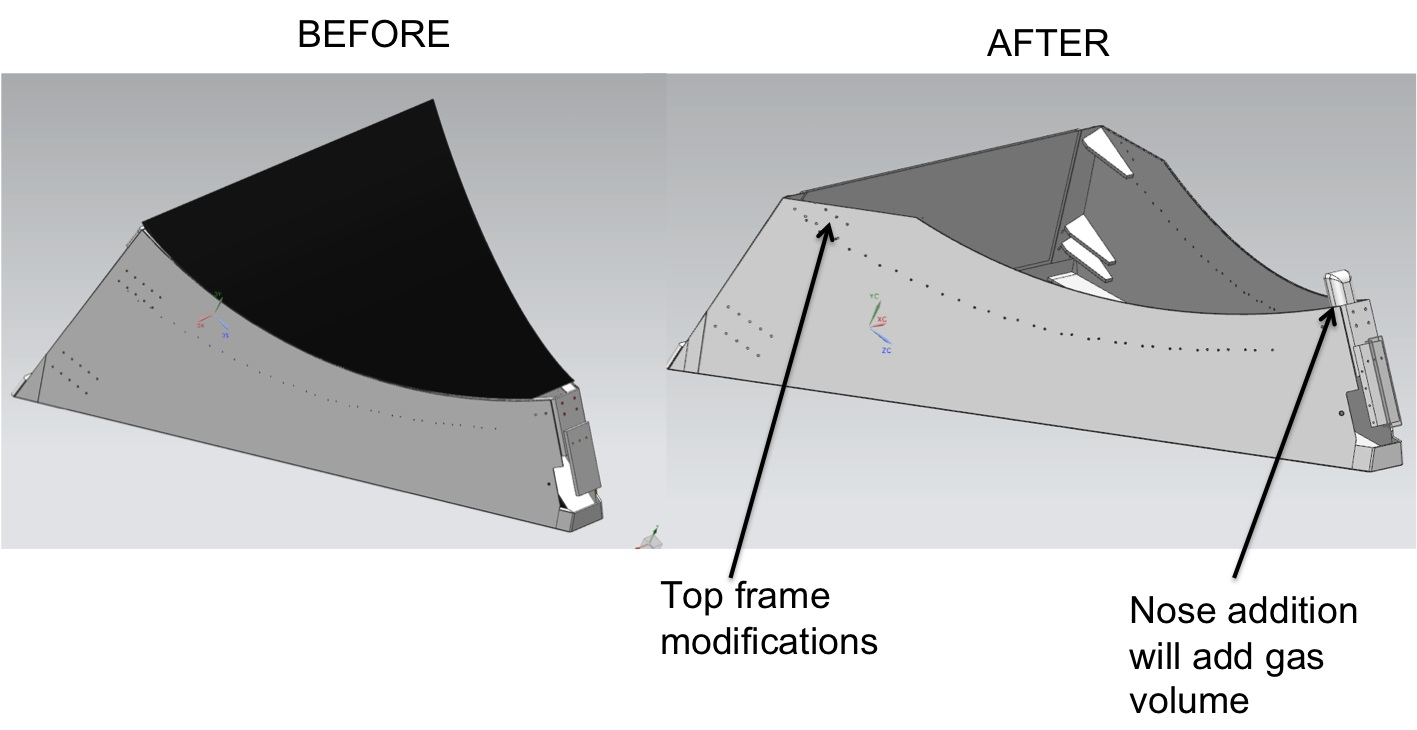
\includegraphics[width=0.98\textwidth]{img/ltcc_mods.jpg}
	\caption{\scriptsize LTCC modifications: cut of the side walls and nose to increase gas volume.}
	\label{fig:mods}
\end{figure}


\begin{figure}[ht]
	\centering
	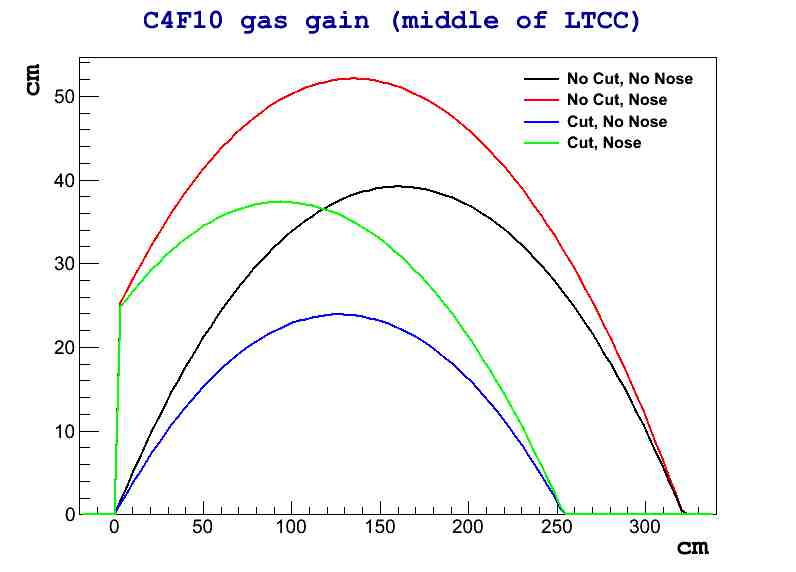
\includegraphics[width=0.98\textwidth]{img/window_addition_gain.jpg}
	\caption{\scriptsize Linear Increase in C4F10 space}
	\label{fig:window}
\end{figure}

\begin{thebibliography}{mybib}
 \bibitem{bib:c4f10refr}    {T.A. Filippas, E. Fokitis, S. Maltezos, K. Patrinos, M. Davenport},   {\refj Nuclear Instruments and Methods in Physics Research B        }        {\bf 196},             340   (2002).
 \bibitem{bib:ccnim}    {G. Adams, V. Burkert et al },   {\refj Nuclear Instruments and Methods in Physics Research A       }        {\bf 465},             414   (2001).
 \bibitem{bib:tamm} {I. Tamm},   {\refj J. Phys. U.S.S.R.,        }        {\bf 1},             439   (1939).
 \bibitem{bib:andrew} {Andrew Puckett},   {Private Communication . } 
 \bibitem{bib:alex} {Alex Vlassov},   {Private Communication . } 
 \bibitem{bib:guerra} {Joe Guerra},   {Private Communication . } 
\end{thebibliography}



\end{document}









